\question{Эффект Шоттки. Его влияние на эмиссию электронов}
Эффект Шоттки состоит в возрастании тока в диоде при увеличении напряжения после
выхода в режим насыщения.

Электрон, выходя из металла, попадает в электрическое поле, сформированное
анодным напряжением и изображением электрона в катоде. При этом эффективное
значение работы выхода уменьшается. Исполльзуя уравнение Ричардсона-Дэшмана,
получаем
\[
    j = CT^2\exp\left(-\frac{A-\Delta A}{kT}\right) =
    j_0\exp\left(\frac{\Delta A}{kT}\right).
\]
\begin{figure}[h]
\begin{center}
    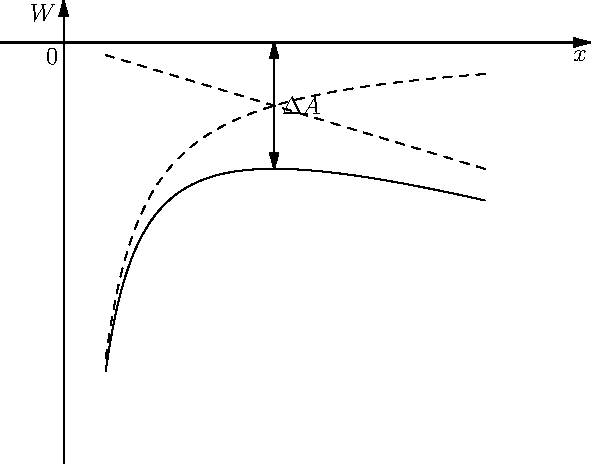
\includegraphics[width=.7\textwidth]{02}
\end{center}
\caption{Профиль энергии электрона вблизи поверхности металла}
\end{figure}

Оценим изменение эффективной работы выхода:
\[
    W = -eEx - \frac{1}{16\pi\eps_0}\frac{e^2}{x},
\]
\[
    \Delta A = -W_{max} = 2eEx_{max} = e\sqrt{\frac{eE}{4\pi\eps_0}}.
\]
Таким образом,
\[
    j = j_0\exp\left(\frac{e}{kT}\sqrt{\frac{e}{4\pi\eps_0}}\sqrt{E}\right).
\]
